
\chapter{模形式与模曲线}
\section{经典模形式回顾}
我们从与模形式密切相关的复环面开始谈起.
\subsection{复环面}

给定$\tau \in \mathcal{H}$,取格点$\Lambda_{\tau}:= \mathbb{Z}\tau \oplus \mathbb{Z} \!\cdot\!\! 1$,则复环面自然成为紧黎曼面,亏格为1.定义\textbf{Weierstrass函数}\footnote{$\sum'$表示对0以外的点求和.}
$$\wp_{\Lambda_{\tau}}(z):=\frac{1}{z^2}+ \summ_{w \in \Lambda_{\tau}}\left( \frac{1}{(z-w)^2}-\frac{1}{w^2} \right)$$
则上述级数在$\mathbb{C} \smallsetminus \Lambda_{\tau}$的紧子集中一致收敛,故$\wp_{\Lambda_{\tau}}(z)$为$\mathbb{C}$上良定的亚纯函数. $\wp_{\Lambda_{\tau}}(z)$有周期$1$, $\tau$, 故$\wp_{\Lambda_{\tau}}$可视作复环面上的亚纯函数.可以证明$\mathbb{C}/\Lambda_{\tau}$上的亚纯函数空间为
$$\mathcal{M}(\mathbb{C}/\Lambda_{\tau})=\mathbb{C}(\wp,\wp') \cong \mathbb{C}(x)[y]/(-y^2+4x^3-g_2x-g_3)\quad g_2,g_3 \in \mathbb{C}. $$

复环面可以通过射影嵌入
$$\mathbb{C}/\Lambda_{\tau} \longrightarrow \mathbb{PC}^2 \qquad \bar{z} \longmapsto \begin{cases}
[\wp,\wp',1], & z \notin \Lambda_{\tau} \\
[0,1,0], & z \in \Lambda_{\tau}
\end{cases} $$
成为$\mathbb{PC}^2$中的射影簇,称为复椭圆曲线.由下图示过程可以得到复环面,亏格为1的紧黎曼面和复椭圆曲线的等价性,详尽解释可参考\cite[第八章]{Li2019modularform}.
\begin{figure}[ht]
	\centering
		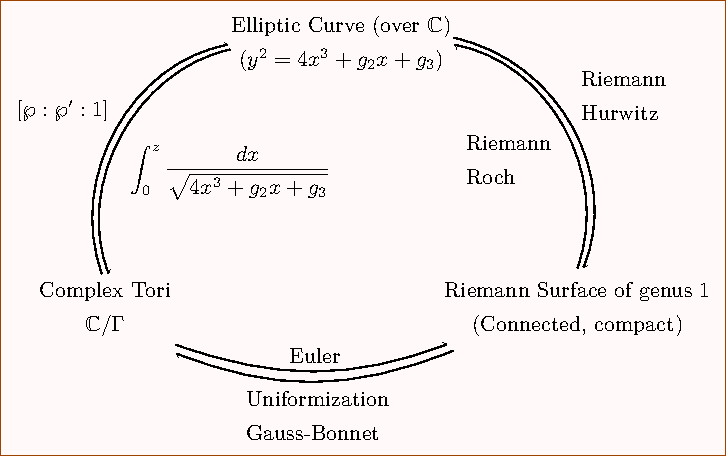
\includegraphics[width=0.8\textwidth]{Flowchart/Ellipticcurve.pdf}
	\label{pic:Ellipticcurve}
\end{figure}

\subsection{模空间$\mathcal{H}/\SL_2(\mathbb{Z})$}
现在我们扰动点$\tau \in \mathcal{H}$,得到不同的复环面.在黎曼面范畴同构的意义下,
$$\Lambda_{\tau} \cong \Lambda_{\tau'} \Longleftrightarrow \text{存在$\gamma \in \SL_2(\mathbb{Z})$,使得$\gamma \tau = \tau'$}$$
故所有复环面构成的空间为$\mathcal{H}/\SL_2(\mathbb{Z})$,在加入尖点紧化后同构于$\mathbb{PC}^1$.为了定义``模空间中的函数(截面)",我们引进模形式的概念:

\begin{defn}
	称$\mathcal{H}$上的全纯函数$f$为权$k \in \mathbb{Z}$,级$\Gamma:= \SL_2(\mathbb{Z})$的模形式,若
	
	\begin{enumerate}[(1)]
		\item 对任意$\gamma=\begin{pmatrix}
		a & b\\
		c & d
		\end{pmatrix}\in \Gamma$,均有
		\begin{equation}\label{eq:modform}
		f(\gamma \tau)=(c \tau +d)^k f(\tau)
		\end{equation}
		特别地,我们有$f(\tau+1)=f(\tau)$.
		\item $f$的Fourier展开$f(\tau)=\sum_{n \in \mathbb{Z}}a_ne^{2\pi i n \tau}$中,对$n < 0$, $a_n =0$.\footnote{一个直观的看法:取$\infty$附近的局部坐标为$q:=\exp(2\pi i \tau)$,则该条件等价于$f$在$\infty$全纯.}
	\end{enumerate}
	记权为$k$,级为$\Gamma$的模形式构成的空间为$\operatorname{M}_k(\Gamma)$, $\operatorname{M}_{*}(\Gamma):= \oplus_{k \in \mathbb{Z}}\operatorname{M}_k(\Gamma)$为对应的分次环.
	
	若额外要求$(2)$中的$a_0=0$ ($\infty$为截影$f$的零点),则称其为尖点形式,及其构成的空间为$\operatorname{S}_k(\Gamma)$, $\operatorname{S}_{*}(\Gamma):= \oplus_{k \in \mathbb{Z}}\operatorname{S}_k(\Gamma)$为对应的分次环.
\end{defn}

\begin{exercise}
	对于$k \in \mathbb{Z}$, $k>2$,定义\textbf{Eisenstein函数}
	$$G_k(\tau):= \frac{1}{2}\summ_{w \in \Lambda_{\tau}} \frac{1}{w^k}=\frac{1}{2} \summ_{(m,n) \in \mathbb{Z}^2} \frac{1}{(m\tau +n)^k}$$
	其中$\sum'$表示对0以外的点求和,可以验证
	\begin{enumerate}
		\item 级数在$\mathcal{H}$的紧子集上一致收敛, $G_k$为$\mathcal{H}$上的全纯函数;
		\item $k$为奇数时, $G_k \equiv 0$;
		\item $k$为偶数时, $G_k$满足\eqref{eq:modform},且有Fourier展开
		$$G_k(\tau)=\frac{(2\pi i)^k}{(k-1)!} \left( -\frac{B_k}{2k}+\sum_{n=1}^{\infty}\sigma_{k-1}(n)q^n \right)$$
		故$G_k$为权$k$,级$\SL_2(\mathbb{Z})$的模形式.
	\end{enumerate}
\end{exercise}

为方便起见,取$E_k:= G_k/(2\zeta(k))$使得Fourier常数项化为1.可以证明, $M_{*}(\SL_2(\mathbb{Z})) \cong \mathbb{C}[E_4,E_6]$,且$E_4,E_6$代数无关.

\begin{remark}
	模形式可视作格点上的函数,即
	$$F: \{\Lambda= \mathbb{Z}e_1 \oplus \mathbb{Z}e_2 \} \longrightarrow \mathbb{C} \qquad \Lambda \longmapsto F(\Lambda)$$
	满足$F(\lambda \Lambda)= \lambda^{-k} F(\Lambda)$
	
	取$f(\tau):=F(\Lambda_{\tau})$,则有
	\begin{equation*}
	\begin{aligned}
	f(\gamma \tau) =\, & F(\Lambda_{\gamma\tau})=F(\mathbb{Z}\gamma\tau \oplus \mathbb{Z} \!\cdot\!\! 1)\\
	=\,& (c\tau + d)^k F\big(\mathbb{Z}(a\tau+b) \oplus \mathbb{Z}(c\tau +d)\big)		\\
	=\,& (c\tau + d)^k F(\Lambda_{\tau})		\\
	=\,& (c\tau + d)^k f(\tau)		\\
	\end{aligned}
	\end{equation*}
	事实上,我们也是通过上述方式来构造Eisenstein级数的.
\end{remark}
\begin{figure}[ht]
		\centering
		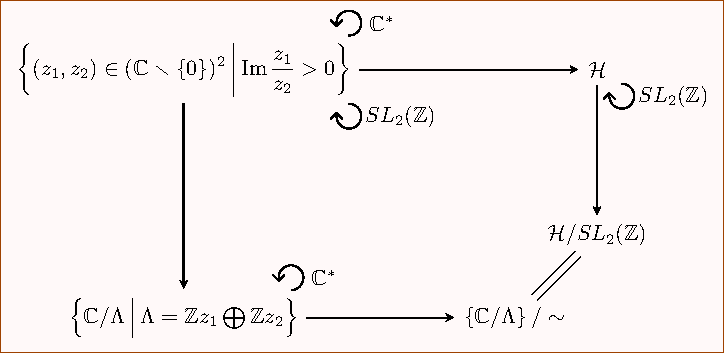
\includegraphics[width=0.8\textwidth]{Flowchart/Modularcurve.pdf}
	\caption{构造模空间/模形式的过程}
	\label{pic:Modularcurve}
\end{figure}
另外补充两个重要的函数:模判别式
$\Delta:=\frac{1}{1728}(E_4^3-E_6^2)$
给出了第一个在$\infty$处取0的模形式,由它可以得到尖点形式的结构;$j:=E_4^3/\Delta$给出紧化的模空间$\mathcal{H}^*/\SL_2(\mathbb{Z})$至$\mathbb{PC}^1$的黎曼面同构.\footnote{注意$j$不是模形式,它在$\infty$处有1阶极点.}

我们以一个表\ref{tb:torus-moduli}作为上述内容的总结:
\begin{table}[ht]
	\centering
	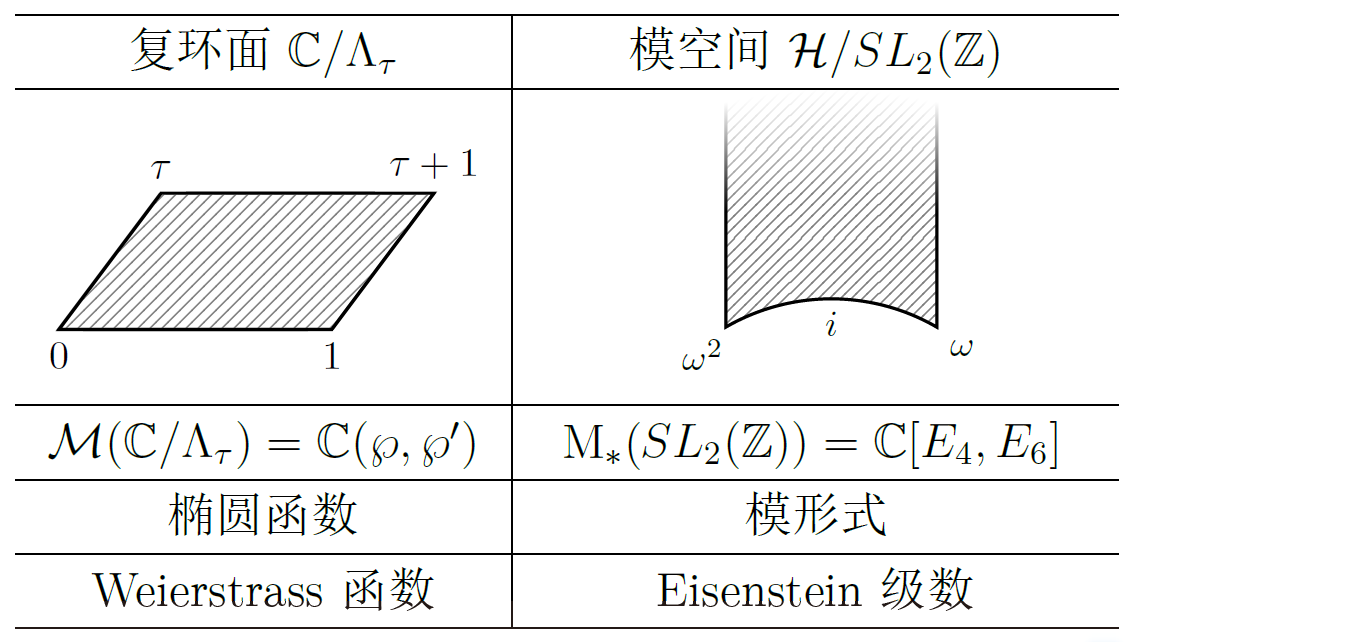
\includegraphics[width=0.6\textwidth]{snip/revised-table-torus-moduli.png}
	\caption{复环面与模空间的比较}
	\label{tb:torus-moduli}
\end{table}
\subsection{Jacobi模形式}
曾经我突发奇想,是否存在一个$\mathcal{H}/\SL_2(\mathbb{Z})$上的纤维丛$E$,使得每一个点$\tau$对应的纤维$E_\tau$恰好就是复环面$\mathbb{C}/\Lambda_{\tau}$?直到有一天我找到了梦中的空间:\footnote{这个空间是$E:=(\mathbb{Z}^2 \rtimes \SL_2(\mathbb{Z})) \textbackslash (\mathcal{H} \times \mathbb{C})$, 其中半直积如下群作用定义:
$$\SL_2(\mathbb{Z})  \times \mathbb{Z}^2 \longrightarrow \mathbb{Z}^2 \qquad \left( \gamma,\rule{0mm}{3.7mm} (m,n) \right) \longmapsto (m,n) \gamma^{-1} .$$
然而,如果你仔细验证的话会发现,每一个点$\tau$对应的纤维$E_\tau$是复环面$\mathbb{C}/\Lambda_{\tau}$商去对径点,即$\mathbb{P}^1$.事实上,由于稳定子群非平凡,$\mathcal{H}/\SL_2(\mathbb{Z})$无法成为细模空间。
}
$$E:=\SL_2(\mathbb{Z})\textbackslash (\mathcal{H} \times \mathbb{C})/\mathbb{Z}^2 \qquad \gamma(\tau,z):= (\gamma \tau,\frac{z}{c\tau +d}) \quad (m,n)(\tau,z):=(\tau, z+m\tau+n)$$
这个空间鼓励我们通过整体的方式来看问题,让我们回顾Weierstrass函数$\wp(z,\tau):= \wp_{\Lambda_{\tau}}(z)$,发现它可以视作两个变元的函数,并且它的Laurent展开
$$\wp(z,\tau)=\frac{1}{z^2}+ \sum_{k=1}^{\infty}(2k+1) G_{2(k+1)}(\tau)z^{2k}$$
中的系数即是经典的模形式.或许作为Weierstrass函数也可以称作某种特殊的模形式?在下一节我们将给出Weierstrass函数的一系列``同类"——$\theta$-函数,它们被统称为Jacobi模形式.
%\begin{defn}
%	我们称亚纯函数$f:\mathbb{C} \times \mathcal{H} \longrightarrow \mathbb{C}$为Jacobi模形式,若
%	\begin{enumerate}[1.]
%		$f$
%	\end{enumerate}
%\end{defn}

%引入向量丛,
%老话常谈的材料中要加入Weierestrass函数的展开是Jacobi模形式,这也是某个$\theta$函数,意味着我们开始讨论“所有复环面”
%Jacobi模形式的定义

\subsection{级结构}
下一步,我们要推广模形式的定义,考虑复环面的级结构,将级从$\SL_2(\mathbb{Z})$推广到同余子群
$$\Gamma(N):=\left\{ \begin{pmatrix}
a &b \\ c & d
\end{pmatrix} \in \SL_2(\mathbb{Z}) \;\middle|\; \begin{pmatrix}
a &b \\ c & d
\end{pmatrix} \equiv \begin{pmatrix}
1 &0 \\ 0 & 1
\end{pmatrix} \mod N  \right\}$$
上. (还记得上章末尾留的任务吗?)简要一提,这个群有一个经典的正合列: ($N>3$)
\begin{center}
	\begin{tikzcd}
		1 \arrow[r]           & \Gamma(N) \arrow[r]             & \PSL_2(\mathbb{Z}) \arrow[r]   & \PSL_2(\mathbb{Z}/N\mathbb{Z}) \arrow[r] & 1 
	\end{tikzcd}
\end{center}

我们定义$\mathcal{H}/\Gamma(N)$的尖点为$\mathbb{PQ}^1 /\Gamma(N)$,有一些不太显然的性质\footnote{参考\cite[练习1.4.14,2.5,例4.2.2]{Li2019modularform}}:
\begin{itemize}
	\item 我们有群的阶数
	$$\mu(N):= \# \,\PSL_2(N) =\begin{cases}\displaystyle
	\frac{N^3}{2} \prod_{p \mid N}(1-p^{-2}), & N>2\\
	6, & N=2
	\end{cases}$$
	\item $N>1$时, $\Gamma(N)$无椭圆点,复叠映射$\mathcal{H} \longrightarrow\mathcal{H}/\Gamma(N)$为非分歧映射; $\mathcal{H}/\Gamma(N)$在标准双曲度量下面积为
	$\frac{\pi}{3} \mu$.
	\item $\Gamma(1)=\SL_2(\mathbb{Z})$在$\mathbb{PQ}^1$上的作用可递,故$\mathcal{H}/\Gamma(1)$的尖点为独点集,记为$\infty$.
	\item 模空间$\mathcal{H}/\Gamma(N)$加入所有尖点后成为紧黎曼面,亏格为
	$$g(N)=\begin{cases}\displaystyle
	1+ \frac{N^2(N-6)}{24} \prod_{p \mid N}(1-p^{-2}), & N >2\\
	0, & N=2
	\end{cases}$$
	其在$\infty$附近的局部坐标为$q:=\exp(2\pi i \tau/N)$;其他尖点通过$\Gamma(1)$的可递作用表示为$\gamma^{-1} \infty$,附近的局部坐标为$\exp(2\pi i \gamma(\tau)/N)$.
	\item 我们有尖点清晰的代数刻画:记
	$$(\mathbb{Z}/N\mathbb{Z})^2_{\prim}:=\left\{(a,b) \in (\mathbb{Z}/N\mathbb{Z})^2 \middle| (a,b)\text{ 为$N$阶元} \right\}$$
	则有$\Gamma(1)$-等变同构\footnote{需要注意这里对取的代表元有限制,要求$x$, $y$互质.}:( $\phi\big((x,y)\gamma\big)=\gamma^{-1}\phi\big((x,y) \big)$ )
	\begin{equation}\label{eq:cusppointiso}
	\phi\colon\pm\textbackslash(\mathbb{Z}/N\mathbb{Z})^2_{\prim} \longrightarrow \{ \Gamma(N) \text{ 的尖点}\} \qquad \overline{(x,y)} \longmapsto \overline{-y/x}
	\end{equation}
	通过这个同构,可以直接算出所有尖点的位置以及尖点的元素个数
	$$n(N)=\begin{cases}\displaystyle \;
	\frac{N^2}{2}  \prod_{p \mid N} (1-p^{-2}), & N >2\\
	\;\;3, & N=2
	\end{cases}$$
\end{itemize}
	在之后,我们记$Y(\Gamma(N)):= \mathcal{H}/\Gamma(N)$, $X(\Gamma(N))$为$Y(\Gamma(N))$紧化后得到的复黎曼面.
\begin{remark}
	类似于$\mathcal{H}/\SL_2(\mathbb{Z})$,可以证明$Y(\Gamma(N))$分类了对象
	$$(\Lambda, \alpha: (\mathbb{Z}/N\mathbb{Z})^2\overset{\sim}{\longrightarrow} E_{\Lambda}[N] )/\sim$$
	其中$E_{\Lambda}[N]:=\left\{ z \in \mathbb{C}/\Lambda \middle| Nz=0 \right\}$, $\alpha$需要满足Drinfeld条件:存在$P,Q \in \frac{1}{N}\Lambda$使得
	$$\bar{P}=\alpha(1,0),\quad \bar{Q}=\alpha(0,1),\quad \Lambda=\mathbb{Z}P \oplus \mathbb{Z}Q,\quad \Img \frac{P}{Q}>0.$$
\end{remark}



\begin{defn}
	称$\mathcal{H}$上的全纯函数$f$为权$k \in \mathbb{Z}$,级$\Gamma:= \Gamma(N)$的模形式,若
	
	\begin{enumerate}[(1)]
		\item 对任意$\gamma=\begin{pmatrix}
		a & b\\
		c & d
		\end{pmatrix}\in \Gamma$,均有
		\begin{equation}\label{eq:modform2}
		f(\gamma \tau)=(c \tau +d)^k f(\tau)
		\end{equation}
		特别地,我们有$f(\tau+N)=f(\tau)$.
		\item $f$在所有尖点处全纯.
	\end{enumerate}
	记权为$k$,级为$\Gamma$的模形式构成的空间为$\operatorname{M}_k(\Gamma)$, $\operatorname{M}_{*}(\Gamma):= \oplus_{k \in \mathbb{Z}}\operatorname{M}_k(\Gamma)$为对应的分次环.
	
	若额外要求函数$h$在所有尖点处消没,则称其为尖点形式,及其构成的空间为$\operatorname{S}_k(\Gamma)$, $\operatorname{S}_{*}(\Gamma):= \oplus_{k \in \mathbb{Z}}\operatorname{S}_k(\Gamma)$为对应的分次环.
\end{defn}
\begin{remark}
	事实上我们需要的定义比这广泛得多:我们将考虑带特征的半整权模形式,并将尖点处要求放松为``极点"\footnote{我们之后只会考虑这个空间具体的函数和特殊的子空间,其在尖点处的性质均可以计算,故定义的空间再大一些也无所谓.}.读者可以将其同第\ref{sec:inva}节中的$\Gamma'$-半不变量作类比.
\end{remark}
\begin{defn}
	称$\mathcal{H}$上的全纯函数$f$为权$k \in \frac{1}{2}\mathbb{Z}$,级$\Gamma:= \Gamma(N)$,特征$\bigchi$的模形式,若对任意$\gamma=\begin{pmatrix}
	a & b\\
	c & d
	\end{pmatrix}\in \Gamma$,均有
	\begin{equation}\label{eq:modform3}
	f(\gamma \tau)=\bigchi(\gamma)(c \tau +d)^k f(\tau)
	\end{equation}
\end{defn}
\begin{remark}
	当$k \in \frac{1}{2} \mathbb{Z} \smallsetminus \mathbb{Z}$时, $(c\tau+d)^k$开根的问题可以被``吸附"至特征$\bigchi$中,故我们只需取一个一致的单值解析分支使得$1^{1/2}=1$即可.\footnote{这个单值解析分支也是唯一的,注意到$c\tau+d \in \mathcal{H}$.}
\end{remark}
%然后重点是提出主同余子群,略述其定义、模空间紧化、尖点的内容,



%直接承认无椭圆点,,指数,亏格公式和尖点个数,列表.

\section{$\theta$-函数}
\subsection{定义}
作为研究经典模形式的有力武器,同时也作为Jacobi模形式的极典型例子,我们引入$\theta$-函数的定义:

\begin{defn}
	我们定义带特征$\chi:=\normalcharacter \in \mathbb{R}^2$的$\theta$-函数
	$$\theta\normalcharacter : 
	\mathbb{C} \times \mathcal{H} \longrightarrow \mathbb{C}$$
	$$\theta\normalcharacter(z, \tau)=\sum_{n \in \mathbb{Z}} \exp 2 \pi i \left\{\frac{1}{2}\left(n+\frac{\epsilon}{2}\right)^{2} \tau+\left(n+\frac{\epsilon}{2}\right)\left(z+\frac{\epsilon^{\prime}}{2}\right)\right\}$$
	
	注意到$\theta$-函数的良定性,且分别关于$z$, $\tau$全纯.
\end{defn}
\subsection{恒等式}
我们在此处不加证明地引用$\theta$-函数的一部分恒等式,这些恒等式的导出均初等,却需要足够的代数成熟度.在这里我们强烈建议对证明感兴趣的读者按着\cite[Chapter2.1]{farkas2001theta}中的步骤一步步推导.
\subsubsection{基本公式}
\begin{gather*}
\intertext{关于$\chi$:}
\theta\normalcharacter(z, \tau)=\exp 2 \pi  i \left\{\frac{1}{8} \epsilon^{2} \tau+\frac{1}{2} \epsilon z+\frac{1}{4} \epsilon \epsilon^{\prime}\right\} \theta\character{0}{0}\left(z+\frac{\epsilon^{\prime}}{2}+\frac{\epsilon}{2} \tau, \tau\right) \tag*{[2.3]} \label{eq:chieq}\\
\theta \character{\epsilon+2m}{\epsilon'+2n}(z,\tau)=\exp(\pi i \epsilon n)\, \theta \normalcharacter (z,\tau)\tag*{[2.9]} \\
	\theta \character{-\epsilon}{-\epsilon'}(z,\tau)= \theta \normalcharacter(-z,\tau)	
\tag*{[2.10]}
\end{gather*}
\begin{gather*}
\intertext{关于$(z)$的平移:\footnotemark}
\theta\normalcharacter(z+n+m \tau, \tau)=\exp 2 \pi  i \left\{\frac{n \epsilon-m \epsilon^{\prime}}{2}-m z-\frac{m^{2}}{2} \tau\right\} \theta\normalcharacter(z, \tau) \tag*{[2.4]}\label{eq:Translation}
\end{gather*}
\footnotetext{$n,m \in \mathbb{Z}$.}
\begin{gather*}
\intertext{关于$(\tau)$的变换公式:\footnotemark}
%\frac{\exp \pi  i \left\{\frac{-c z^{2}}{c \tau+d}\right\} \theta\normalcharacter\left(\frac{z}{c \tau+d}, \frac{a \tau+b}{c \tau+d}\right)}{\theta \character{a \epsilon+c \epsilon^{\prime}-a c}{b \epsilon+d \epsilon^{\prime}+b d}(z, \tau)}=\kappa\left(\normalcharacter, \gamma\right)(c \tau+d)^{\frac{1}{2}}
\hspace{-3cm}\theta\normalcharacter\left(\frac{z}{c \tau+d}, \frac{a \tau+b}{c \tau+d}\right) =\kappa\left(\normalcharacter, \gamma\right)(c \tau+d)^{\frac{1}{2}} \\
\hspace{3cm}\times \exp \pi  i \left\{\frac{c z^{2}}{c \tau+d}\right\} \theta \character{a \epsilon+c \epsilon^{\prime}-a c}{b \epsilon+d \epsilon^{\prime}+b d}(z, \tau)
\tag*{[2.16]}\label{eq:Transformation}
\intertext{其中$\kappa\left(\character{0}{0}, \gamma \right)$为八次单位根,只依赖于$\gamma$;而}
\hspace{-8cm}\kappa\left(\normalcharacter, \gamma\right)= \kappa\left(\character{0}{0}, \gamma\right) \\
\hspace{3cm}\times\exp 2 \pi  i \left\{-\frac{1}{4}\left(a \epsilon+c \epsilon^{\prime}\right) b d-\frac{1}{8}\left(a b \epsilon^{2}+c d \epsilon^{\prime 2}+2 b c \epsilon \epsilon^{\prime}\right)\right\}  \tag*{[2.17]}\label{eq:Transformation2}
\end{gather*}

\footnotetext{$\gamma=\left(\begin{smallmatrix}
	a & b\\ c & d
	\end{smallmatrix}\right) \in \SL_2(\mathbb{Z})$}
\subsubsection{方程相关公式}
\begin{gather*}
\intertext{函数方程:($\theta$-函数的另一种定义)固定$\tau$, $\chi$,令$f(z):=\theta \normalcharacter(z,\tau)$,则}
f(z+1, \tau)=\exp (\pi  i  \epsilon) f(z, \tau) 	\tag*{[2.5]}\\
f(z+\tau, \tau)=\exp \left(-\pi  i \left\{\epsilon^{\prime}+2 z+\tau\right\}\right) f(z, \tau)	\tag*{[2.6]}	
\intertext{热方程(物理意义):简记$':=\partial_z$,则}
\theta'' \normalcharacter (z,\tau) =4\pi i \frac{\partial \theta}{\partial \tau} \normalcharacter (z,\tau)	\tag*{[p73]}
\intertext{Fourier展开:记$w:=\exp (2\pi iz)$,则}	
\theta \normalcharacter (z,\tau) =\omega^{\textstyle\frac{\epsilon}{2}} \sum_{n\in \mathbb{Z}}a_n\omega^n	\tag*{[2.7]}
\intertext{其中}
a_{n}=\exp 2\pi i \left\{ \frac{1}{2} \left(n+\frac{\epsilon}{2}\right)^2 \tau + \left(n+\frac{\epsilon}{2}\right) \frac{\epsilon'}{2}  \right\}
\end{gather*}

\subsubsection{乘积公式}
记$w:=\exp (2\pi iz)$, $q=\exp (2\pi i \tau)  $,则\footnote{在许多书中均取$q=\exp \{\pi i \tau \}$,但我们统一取$q=\exp \{2 \pi i \tau\}$,希望读者不要混淆.}
\begin{equation*}
	\begin{aligned}
	\theta \character{0}{0}(z,\tau)=\;& \sum_{n \in \mathbb{Z}}q^{\frac{n^2}{2}}w^n\\
	=\;& \prod_{n=1}^{\infty}(1-q^n)\left( 1+q^{\frac{2n-1}{2}}w \right) \left( 1+\frac{q^{\frac{2n-1}{2}}}{w} \right)
	\end{aligned}
\end{equation*}
作为推论,我们有
$$\sum_{n \in \mathbb{Z}} (-1)^n x^{\frac{kn^2+ln}{2}}=\prod_{n=0}^{\infty} \left(1-x^{kn+\frac{k-l}{2}} \right)\left(1-x^{kn+\frac{k+l}{2}} \right)\left(1-x^{kn+k} \right)$$
并且由\ref{eq:chieq},所有的$\theta$-函数均有对应的乘积公式。
\subsubsection{散在恒等式}
%在书中还有一些散在恒等式,也在此一并列下:
\begin{gather*}
\theta\normalcharacter(z, \tau)=\sum_{l=0}^{N-1} \theta\character{\frac{\epsilon+2 l}{N}}{N \epsilon^{\prime}}\left(N z, N^{2} \tau\right)	\tag*{[p76]} \\
\theta\normalcharacter(0, \tau) \theta\character{\delta}{ \delta^{\prime}} (0, \tau)   =\theta\character{\frac{\epsilon+\delta}{2}} {\epsilon^{\prime}+\delta^{\prime}} (0,2 \tau) \theta\character{\frac{\epsilon-\delta}{2}}   {\epsilon^{\prime}-\delta^{\prime}} (0,2 \tau)\\
\hspace{6.5cm}   +\theta\character{\frac{\epsilon+\delta}{2}+1}   {\epsilon^{\prime}+\delta^{\prime}} (0,2 \tau) \theta\character{\frac{\epsilon-\delta}{2}+1}   {\epsilon^{\prime}-\delta^{\prime}} (0,2 \tau)	\tag*{[2.15]} \\
\theta \normalcharacter (-z,\tau) =\exp (\pi i \epsilon \epsilon') \theta \normalcharacter (z,\tau) \qquad \text{当$\normalcharacter \in \mathbb{Z}^2$}	\tag*{[p76]} 
\end{gather*}
\begin{remarks}\
	\begin{enumerate}[1.]
		\item 含参是为了有更多的操作空间,取不同的特殊值则能得到更多更简洁优美的恒等式.例如,令$z=0$,我们得到\textbf{$\theta$-级数}\footnote{我们使用相同的符号,注意不要混淆.}:
		$$\theta \normalcharacter (\tau):=\theta \normalcharacter (0,\tau)$$
		特别地, $\theta \character{0}{0}$, $\theta \character{1}{0}$, $\theta \character{0}{1}$, $\theta \character{1}{1} \equiv 0$是人们所熟知的\textbf{Jacobi $\theta$-级数},例如:
		$$\theta \character{0}{0} (\tau) = \sum_{n \in \mathbb{Z}} q^{\textstyle \frac{n^2}{2}}=1+2q^{\textstyle \frac{1}{2}}+2q^{2} + 2q^{\textstyle \frac{9}{2}}+ \cdots$$
		我们简记其为$\theta_{00}(\tau)$, $\theta_{10}(\tau)$, $\theta_{01}(\tau)$, $\theta_{11}(\tau)$,它们之间有关系
		$$\theta_{00}^4=\theta_{01}^4+\theta_{10}^4$$
		
		有时我们也会用到含参数的Jacobi $\theta$-函数$\theta_{00}(z,\tau)$, $\theta_{10}(z,\tau)$, $\theta_{01}(z,\tau)$, $\theta_{11}(z,\tau)$,注意到他们都是关于$z$的奇/偶函数,这一点有助于在之后极大地简化计算过程(Taylor展开有一半为0).
		\item $\theta$函数除了拥有丰富的恒等式外,作为$z$的函数(固定$\chi, \tau$), $\theta \normalcharacter (z,\tau)$仅在$\displaystyle\frac{1-\epsilon'}{2}+\frac{1-\epsilon}{2}\tau + \Lambda_{\tau}$处有一阶零点.它同样可视作$\mathbb{C}/\Lambda_{\tau}$上某个向量丛的截影.这使得我们可以通过$\theta$函数来构造众多的模形式.
		\begin{table}[ht]
			\centering
			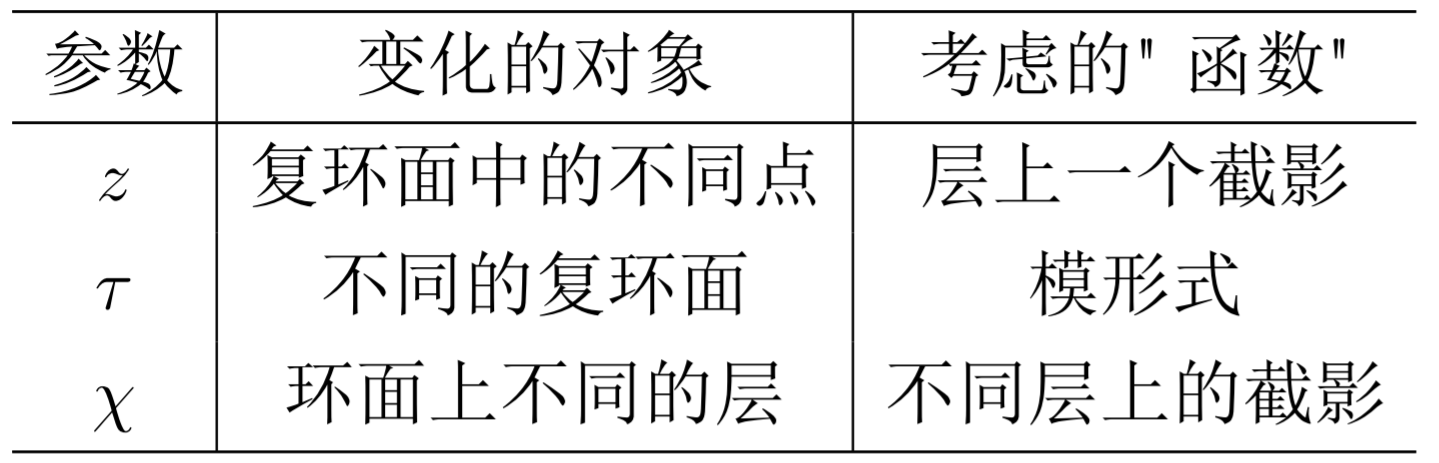
\includegraphics[width=0.5\textwidth]{snip/table-geomean.png}
			\caption{参数所代表的几何意义}
		\end{table}
		\item 恒等式不只是恒等式,它们有丰富的几何/算术性质.通过这种观点,我们将通过这些恒等式给出$X(\Gamma(N))$的性质.
	\end{enumerate}
	
\end{remarks}
%第二节引用,提出$\theta$函数,直接抄材料里的恒等式
\subsection{应用:表达$\wp$, $G_4$和$G_6$}
%小试牛刀,我们试着用$\theta$-函数来表达$\wp$, $G_4$和$G_6$.

\begin{theorem}[{\cite[Chapter 2, Theorem 5.10]{farkas2001theta}}]
	我们有表达
	\begin{equation}\label{eq:wpwiththeta}
	\wp_{\Lambda_{\tau}}(z) = - \left(\frac{\thetaaa{'}{z,\tau}}{\thetaaa{}{z,\tau}}\right)' +\frac{1}{3} \frac{\thetaaa{(3)}{0,\tau}}{\thetaaa{'}{0,\tau}}
	\end{equation}
\end{theorem}
\begin{proof}
	右式只在$\Lambda_{\tau}$处有二阶极点,比较两边在$0$处的Laurent展开即得.
\end{proof}
\begin{corollary}
	比较\eqref{eq:wpwiththeta}式两边系数得
	\begin{equation*}
	\begin{aligned}
	E_4(\tau)=\;&\frac{1}{18} \left(\frac{\thetaaatau{(3)}}{\thetaaatau{'}} \right)^2-\frac{1}{30} \frac{\thetaaatau{(5)}}{\thetaaatau{'}}\\
	E_6(\tau)=\;& \frac{1}{120} \frac{\thetaaatau{(3)}\thetaaatau{(5)}}{\thetaaatau{'}^2}-\frac{1}{108} \left(\frac{\thetaaatau{(3)}}{\thetaaatau{'}} \right)^3-\frac{1}{840} \frac{\thetaaatau{(7)}}{\thetaaatau{'}}
	\end{aligned}
	\end{equation*}
	$\Delta$, $j$亦可用$\theta$-级数表达.
\end{corollary}
\begin{exercise}
	固定$\tau \in \mathcal{H}$,试验证
	$$\mathbb{C}/\Lambda_{\tau} \longrightarrow \mathbb{PC}^2 \qquad z \longmapsto \left[\theta_{00}^2\theta_{11},\theta_{00}\theta_{01}\theta_{10},\theta_{11}^3 \right]$$
	为射影嵌入,得到$\mathbb{PC}^2$中的代数方程
	$$\theta_{00}^4 Y^2Z=X(\theta_{10}^2X-\theta_{01}^2Z)(\theta_{01}^2X+\theta_{10}^2Z).$$
\end{exercise}

%???然后把4个特殊的$\theta$函数列出来,说明其特殊性质(奇偶性(Taylor展开),四次恒等式,Jacobi导数公式,用$\theta$函数表示Weierestrass函数以及模形式,重新描述射影嵌入)
%还有$\eta$函数和乘积公式也可以顺手一提
%
%???Jacobi三/五乘积公式


\section{构造模形式}\label{sec:consofmodularform}

当我们想要进一步探讨如何用$\theta$-级数表达主同余子群的模形式时,一定会重新将焦点转移至公式\ref{eq:Translation}上.记$\chi:=\normalcharacter$, $\chi\gamma:=\character{a\epsilon+c\epsilon'-ac}{b\epsilon+d\epsilon'+bd}$,我们用更简练的语言来重新表达公式\ref{eq:Transformation}:
$$\exp \pi i \left\{ -cz^2\gamma'(\tau)^{\frac{1}{2}} \right\}\theta[\chi](z\gamma'(z)^{\frac{1}{2}},\gamma(\tau))=\kappa(\chi,\gamma)\gamma'(\tau)^{-\frac{1}{4}} \theta[\chi\gamma] (z,\tau)$$
取$z=0$,则有
\begin{equation}\label{eq:Transformation3}
\theta[\chi](0,\gamma(\tau))=\kappa(\chi,\gamma)\gamma'(\tau)^{-\frac{1}{4}} \theta[\chi\gamma] (0,\tau)
\end{equation}
当$\chi \gamma=\chi$时, $\theta[\chi](0,-)$成为权$1/2$,特征为$\kappa(\chi,-)$的模形式,然而这是在做梦.退而求其次,当$\chi\gamma \equiv \pm \chi \;(\!\!\!\!\mod (2\mathbb{Z})^2)$时,我们可以通过\ref{eq:Transformation2}调整公式\ref{eq:Translation},得到$\theta[\chi](0,\gamma(\tau))$同$\theta[\chi](0,\tau)$的关系.
\subsection{等价特征类空间}
\begin{defn}
	我们称特征类$\chi$与$\chi'$等价,若$\chi \equiv \pm \chi' \;(\!\!\!\!\mod (2\mathbb{Z})^2)$,记等价特征类的空间为$\mathds{X}:=\mathbb{R}^2/\sim$.
\end{defn}
\begin{figure}[ht]
	
	\begin{minipage}[t]{.9\textwidth}
		\vspace{0.1cm}
		\centering
		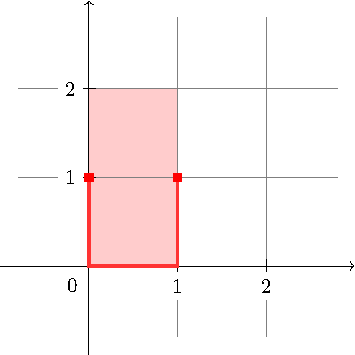
\includegraphics{pic/funsetofchar.pdf}
		
	\end{minipage}
	\caption{$\mathds{X}$所对应的基本集}
	\label{pic:basicsetofchar}
\end{figure}
\begin{defn}
	定义$\Gamma(1)$在$\mathds{X}$上的右作用
	$$\mathds{X} \times \Gamma(1) \longrightarrow \mathds{X} \qquad \normalcharacter \gamma := \character{a\epsilon+c\epsilon'-ac}{b\epsilon+d\epsilon'+bd}$$
	由于
	\begin{equation*}
	\begin{aligned}
	\normalcharacter \gamma =& \character{a(\epsilon-1)+c(\epsilon'-1)+a+c-ac-1+1}{b(\epsilon-1)+d(\epsilon'-1)+b+d+bd+1-2+1}\\
	=& \begin{pmatrix}
	a & c \\ b & d
	\end{pmatrix}
	\character{\epsilon-1}{\epsilon'-1}+\character{-(a-1)(c-1)}{(b+1)(d+1)-2}+\character{1}{1}\\
	\footnotemark\equiv &\footnotemark\gamma^T \left(\chi-\character{1}{1}\right)+\character{1}{1}\\
	& \Longrightarrow \chi\gamma-\character{1}{1}=\gamma^T\left(\chi-\character{1}{1}\right)
	\end{aligned}
	\end{equation*}
	\footnotetext{$a$, $c$不可同时为偶数,故$(a-1)(c-1)$为偶数.}
	故这确实是良定的群作用.
\end{defn}
\begin{remark}
	记$e_1=\character{1}{0}$, $e_2=\character{0}{1}$, $e_3=\character{0}{0}$, $e_4=\character{1}{1}$,则对任意$\gamma \in \Gamma(1)$,有
	\begin{itemize}
		\item $e_4\gamma=e_4$;
		\item $\gamma$诱导了$e_1,e_2,e_3$的一个置换.
	\end{itemize}
\end{remark}
\subsection{二次描述尖点}
\begin{theorem}[{\cite[Chapter 2, 2.6]{farkas2001theta}}]
	回顾$\Gamma(N)$的尖点同$\pm\textbackslash(\mathbb{Z}/N\mathbb{Z})^2_{\prim}$的一一对应.定义
	$$\iota\colon \pm\textbackslash(\mathbb{Z}/N\mathbb{Z})^2_{\prim} \longrightarrow \mathds{X} \qquad \overline{(x,y)} \longmapsto \character{\frac{N-2x}{N}}{\frac{N-2y}{N}}$$
	则$\iota$为$\Gamma(1)$-等变的嵌入映射,记$X_0(N):=\Img \iota$,则有尖点同$X_0(N)$的一一对应,且$\Gamma(1)$在$X_0(N)$上的作用可递.
\end{theorem}
\begin{example1}
	直接计算可得到$X_0(1)=\{e_4\}$, $X_0(2)=\{e_1,e_2,e_3\}$.图\ref{pic:cusps}画出了$X_0(5)$及其所对应的尖点.
	
	\begin{figure}[ht]
		\centering
		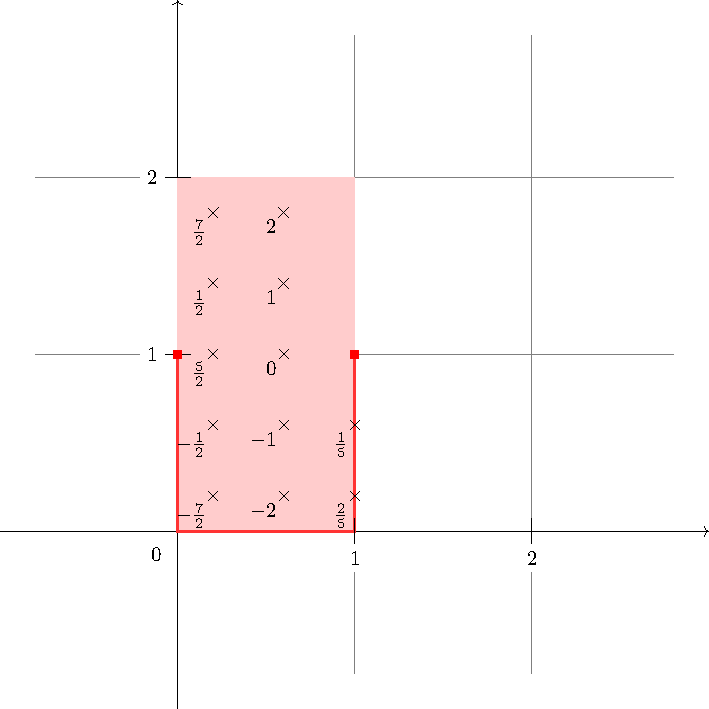
\includegraphics[scale=0.8]{pic/cuspofX(5).pdf}
		\caption{$X_0(5)$}
		\label{pic:cusps}
	\end{figure}
\end{example1}
\begin{theorem}[{\cite[Chapter 2, Lemma 2.7]{farkas2001theta}}]\
	\begin{enumerate}[1.]
		\item $\gamma \in \Gamma(N)$固定$X_0(N)$中的每个点.
		\item 设$\gamma \in \Gamma(1)$固定$X_0(N)$中的每个点,则$\gamma \in \pm\Gamma(N)$.
		%		\item 记$\Perm(X_0(N))$为$X_0(N)$的置换群,我们有群嵌入\vspace{-0.6cm}
		%		$$\PSL_2(\mathbb{Z}/N\mathbb{Z}) \cong \SL_2(\mathbb{Z})/\pm\Gamma(N) \hookrightarrow \Perm(X_0(N))$$\\[-1.8cm]
		%		$\,$
		\item 记$\Perm(X_0(N))$为$X_0(N)$的置换群,我们有群嵌入
		$$\PSL_2(\mathbb{Z}/N\mathbb{Z}) \cong \SL_2(\mathbb{Z})/\pm\Gamma(N) \hookrightarrow \Perm(X_0(N))$$
		\item 设$N>1$,则对每个$\chi \in X_0(N)$, $\theta[\chi]:=\theta[\chi](0,-)$为权$1/2$,特征为$\bigchi$的模形式,其中$\bigchi^{8k} \equiv 1 $.
	\end{enumerate}
	
\end{theorem}
\begin{proof}\
	\begin{enumerate}[1.]
		\item 回顾尖点的定义是$\mathbb{Q}^*/\Gamma(N)$.当然也可以通过计算验证.
		\item 记
		$$\chi_1(N):= \character{1}{\alpha/N} \qquad \chi_2(N):= \character{\alpha/N}{1} \qquad \chi_3(N):= \character{\alpha/N}{\alpha/N}$$
		其中
		$$\alpha=\begin{cases}
		0, & k=2\\
		1, & k\equiv 1 \;(\hspace{-4.2mm}\mod 2)\\
		2, & k\equiv 0 \;(\hspace{-3.8mm}\mod 4)\\
		4, & \text{其他}
		\end{cases}$$
		则$\chi_i(N) \in X_0(N)$,故$\gamma\chi_i(N)=\chi_i(N)$,从而算出$\gamma \in \pm\Gamma(N)$.
		\item 由1.与2.可知.
		\item 记$\chi:=\normalcharacter$, $\chi\gamma=\pm \chi +2nv_1+2n'v_2$,则
		$$\theta[\chi \gamma]=\exp \pi i \left\{ \epsilon n' \right\} \theta[\chi]$$
		代入\eqref{eq:Transformation3}得到
		\begin{equation}\label{eq:Transformation4}
		\theta[\chi](0,\gamma(\tau))=\kappa(\chi,\gamma) \exp \pi i \left\{ \epsilon n' \right\} \gamma'(\tau)^{-\frac{1}{4}} \theta[\chi] (0,\tau)
		\end{equation}
		记$\bigchi(\gamma)=\kappa(\chi,\gamma) \exp \pi i \left\{ \epsilon n' \right\}$,则$\theta[\chi]$为权$1/2$,特征为$\bigchi$的模形式.
	\end{enumerate}
	
\end{proof}

既然给出了模形式的例子,我们自然要关心其在尖点附近的性质.
\begin{defn}
	设$f$是$\mathcal{H}^*:=\mathcal{H} \cup \mathbb{R}^*$的函数, $\xi$为$X(\Gamma(k))$在$z \in \mathbb{R}^*$处的局部坐标,且有展开
	$$f(\tau)= \sum_{x \in \mathbb{R}}a_x\xi^x \qquad \{x \in \mathbb{R} \mid a_x \neq 0  \}\text{ 离散}$$
	则定义$f$在$z$点处的阶为
	$$\ord_zf(\tau):= \inf\{x \in \mathbb{R}\}a_x\xi^x \qquad \{x \in \mathbb{R} \mid a_x \neq 0\}.$$
\end{defn}

取正整数$k>1$,设$\chi=\character{m/k}{m'/k} \in X_0(k)$且$\chi$落在基本集中,注意$X(\Gamma(k))$在$\infty$处附近的局部坐标为$\xi:=\exp 2\pi i \tau/k$,且我们可以将$\theta[\chi]$表达成$\xi$的级数(这可视为$\theta$-级数在$\infty$处的展开),例如
$$\theta\character{m/k}{m'/k}=\xi^{\frac{m^2}{8k}} \sum_{n \in \mathbb{Z}} \exp \pi i \left\{ \frac{mm'}{2k}+\frac{m'n}{k} \right\} \xi ^{\frac{k}{2} n\left(n+\frac{m}{k} \right)}$$
故$\ord_{\infty} \theta[\chi]= \frac{m^2}{8k}$.类似地,我们得到
\begin{equation*}
\begin{aligned}
\ord_{\infty} \theta'[\chi]=& \begin{cases}
\frac{m^2}{8k}, & m \neq 0\\
\frac{k}{2}, & m=0
\end{cases} & \chi \neq \{v_1,v_2,v_3\} \\
\ord_{\infty} \frac{\theta'[\chi]}{\theta[\chi]}=& \begin{cases}
0, & m = 0 \text{ or }k,\; m'<k \\
\frac{k}{2}, & 0<m<k
\end{cases} & \chi \neq X(2) \\
\ord_{\gamma(x)} \theta[\chi](\tau)=&\;\ord_{x} \theta[\chi](\gamma\tau)=\ord_{x} \theta[\chi\gamma](\tau)\\
\ord_{\gamma(x)} \theta'[\chi](\tau)=&\;\ord_{x} \theta'[\chi](\gamma\tau)=\ord_{x} \theta'[\chi\gamma](\tau)\\
\end{aligned}
\end{equation*}


\subsection{$Y(\Gamma(N))$:全纯函数与射影嵌入}

为了具体给出空间$X(\Gamma(N))$上的亚纯函数,乃至于给出$X(\Gamma(N))$的射影嵌入,我们需要两个(或多个)同权同特征的模形式,以下为方便起见,设$N=k$为奇素数\footnote{读者可时刻取$k=5$或$k=7$作为例子,这也是我们故事的终点(不过这显然不是该数学领域的终点).}对$l=0,\ldots,\frac{k-3}{2}$,取$\chi_l:= \character{\frac{2l+1}{k}}{1} \in X_0(k)$,定义全纯函数
$$\varphi_l: \mathcal{H} \longrightarrow \mathbb{C} \qquad \tau \longmapsto \theta[\chi_l](0,k\tau)$$
\begin{theorem}[{\cite[p218]{farkas2001theta}}]
	函数$\varphi_l$ ($l=0,\ldots,\frac{k-3}{2}$)为级$\Gamma(k)$权$1/2$的模形式,且具有相同特征$\bigchi_k$.
\end{theorem}
\begin{proof}
	设
	$$\gamma = \begin{pmatrix}
	a & b \\ c & d
	\end{pmatrix}= \begin{pmatrix}
	a'k+1 & b'k \\ c'k & d'k+1
	\end{pmatrix}\in \Gamma(k), \qquad \hat{\gamma}:=\begin{pmatrix}
	a & bk \\ c/k & d
	\end{pmatrix},$$
	$$\chi_l=\character{t_l}{1}=\character{\frac{2l+1}{k}}{1}, \qquad \chi_l \hat{\gamma} := \chi_l+n_le_1+n_l'e_2,$$
	则有
	\begin{equation*}
	\begin{aligned}
	&\gamma'(\tau)^{\frac{1}{4}}\theta[\chi_l](0,k\gamma(\tau ))\hspace{3mm}\\
	=\hspace{3mm}& \hat{\gamma}'(k\tau)^{\frac{1}{4}}\theta[\chi_l](0,\hat{\gamma}(k\tau ))\\
	\xeq[]{\eqref{eq:Transformation4}}\;& \kappa(\chi_l, \hat{\gamma})\exp \pi i \{ t_ln_l' \} \theta[\chi_l](0,k\tau)		\\
	\end{aligned}
	\end{equation*}
	记$\bigchi_{k,l}(\gamma):=\kappa(\chi, \hat{\gamma})\exp \pi i \{ t_ln_l' \}$,则$\varphi_l$为级$\Gamma(k)$,特征$\bigchi_{k,l}(\gamma)$的模形式.接下来,我们只需计算$n_l'$并证明$\bigchi_{k,l}(\gamma)=\bigchi_{k,l'}(\gamma)$即可.
	
	由于
	$$\chi_l\hat{\gamma}=\character{at_l+\frac{c}{k}-a\frac{c}{k}}{bkt_l+d+bdk}=\character{t_l}{1}+\character{(a-1)t_l+\frac{c}{k}-a\frac{c}{k}}{bkt_l+d+bdk-1}$$
	可验证$(a-1)t_l+\frac{c}{k}-a\frac{c}{k}$, $bkt_l+d+bdk-1 \in 2\mathbb{Z}$,故$n_l'=\frac{1}{2}(bkt_l+d+bdk-1)$,此时
	\begin{equation*}
	\begin{aligned}
	\bigchi_{k,l}(\gamma)=\;& \exp 2\pi i \frac{1}{4} \left\{ -(at_l+\frac{c}{k})bdk-\frac{1}{2} \left( abkt_l^2+\frac{c}{k}d+2bct_l \right) \right\}\\
	& \cdot \exp 2\pi i \frac{1}{4} \left\{ t_l(bkt_l+d+bdk-1)  \right\}\\
	=\;& \exp 2\pi i \frac{1}{4} \left\{ (bk-\frac{1}{2}abk)t_l^2 +(d+bdk-1-abdk-bc)t_l-bcd-\frac{cd}{2k} \right\}
	\end{aligned}
	\end{equation*}
	故只需说明
	\begin{equation*}
	\begin{aligned}
	\frac{1}{4}t_l^2 (bk-\frac{1}{2}abk) \equiv\;&\frac{1}{4}t_{l'}^2 (bk-\frac{1}{2}abk) &(\hspace{-4.3mm}\mod \mathbb{Z})\\
	\frac{1}{4}t_l(d+bdk-1-abdk-bc) \equiv\;& \frac{1}{4}t_{l'}(d+bdk-1-abdk-bc)  &(\hspace{-4.3mm}\mod \mathbb{Z})
	\end{aligned}
	\end{equation*}
	即可,这等价于证明
	\begin{equation*}
	\begin{aligned}
	&(l-l')(l+l'+1)(b'-\frac{1}{2}ab') \in \mathbb{Z}\\
	&\frac{1}{2}(l-l')(d'+bd-abd-b'c'k) \in \mathbb{Z}
	\end{aligned}
	\end{equation*}
	由初等数论知识\footnote{例如, $d'+bd-abd-b'c'k \equiv (d+1) +bd+abd+bc \equiv d+bd+abd+ad \equiv d(a+1)(b+1) \equiv 0 \;\;(\hspace{-2.4mm}\mod 2)$.}可知成立.
\end{proof}
\begin{corollary}
	$\varphi_l/\varphi_{l'}$为$\mathcal{H}/\Gamma(k)$上无零点的全纯函数,且我们有良定的全纯映照
	$$\Phi: \mathcal{H}/\Gamma(k) \longrightarrow \mathbb{PC}^{\frac{k-3}{2}} \qquad \bar{\tau} \longmapsto \left[ \varphi_0(\tau),\ldots , \varphi_{\frac{k-3}{2}}(\tau) \right]$$
\end{corollary}

在接下来的篇幅中,我们将
\begin{itemize}
	\item 延拓$\varphi_l/\varphi_{l'}$至$X(\Gamma(k))$上的亚纯函数并计算其除子;
	\item 延拓$\Phi$至$X(\Gamma(k))$;
	\item 描述$\Gamma(1)$在$\Img \Phi$中的作用(以$\frac{k-1}{2} \times \frac{k-1}{2}$的矩阵表达!),并利用$\Gamma(1)$在尖点集合作用的可递性来找出尖点的像;
	\item 对$k=5,7$,证明$\Phi$为嵌入映射\footnote{然而我不知道一般情况是否如此,书中认为是一个猜想.};
\end{itemize}
\subsection{$X(\Gamma(N))$:尖点与亚纯函数}
为了更方便地观察尖点的性质,我们通过映射
$$\Psi: \mathbb{Q}^*/\Gamma(k) \longrightarrow \mathbb{Q}^*/\Gamma_0(k)$$
将尖点分成两类,其中
$$\Gamma_0(k):=\left\{ \begin{pmatrix}
a &b \\ c & d
\end{pmatrix} \in \SL_2(\mathbb{Z}) \;\middle|\; \begin{pmatrix}
a &b \\ c & d
\end{pmatrix} \equiv \begin{pmatrix}
* & * \\ 0 & *
\end{pmatrix} \mod k  \right\}$$
对偶地定义
$$\Gamma^0(k):=\left\{ \begin{pmatrix}
a & b \\ c & d
\end{pmatrix} \in \SL_2(\mathbb{Z}) \;\middle|\; \begin{pmatrix}
a & b \\ c & d
\end{pmatrix} \equiv \begin{pmatrix}
* & 0 \\ * & *
\end{pmatrix} \mod k  \right\}$$
注意到这两个同余子群之间的共轭同构:
$$\Gamma_0(k) \longrightarrow \Gamma^0(k) \qquad \begin{pmatrix}
a & b \\ c & d
\end{pmatrix} \longmapsto \begin{pmatrix}
a & bk \\ c/k & d
\end{pmatrix}$$
\begin{lemma}\
	\begin{enumerate}[(1)]
		\item $\mathbb{Q}^*/\Gamma_0(k)=\{\bar{\infty}, \bar{0} \}$.换句话说,对任意$r \in \mathbb{Q}^*$,存在$\gamma \in \Gamma_0(k)$,使得$\gamma (0)=r$或$\gamma (\infty)=r$;
		\item $$\Psi^{-1}(\bar{\infty})= \left\{ \Gamma(k) \frac{2l+1}{k} \;\middle|\; l=0,\ldots,\frac{k-3}{2} \right\}$$
		\item 对$\gamma=\left(\begin{smallmatrix}
		a & b \\ c & d
		\end{smallmatrix}\right) \in \Gamma_0(k)$,记$\hat{\gamma}\left(\begin{smallmatrix}
		a & bk \\ c/k & d
		\end{smallmatrix}\right)$,则存在置换$\sigma_{\gamma} \in \Perm \{0,\ldots,\frac{k-3}{2} \}$与特征$\tilde{\kappa}(\chi_l,-):\Gamma^0(k) \longrightarrow \mathbb{C}^*$,使得
		$$\gamma^{\frac{1}{4}}(\tau)\varphi_l(\gamma\tau)=\tilde{\kappa}(\chi_l,\hat{\gamma})\varphi_{\sigma_{\gamma}(l)}(\tau) $$
	\end{enumerate}
	
\end{lemma}
\begin{proof}\
	\begin{enumerate}[(1)]
		\item 记$\gamma=\left(\begin{smallmatrix}
		a & b \\ c'k & d
		\end{smallmatrix}\right)$,则$\gamma (0)=\frac{b}{d}$, $\gamma (\infty)=\frac{a}{c'k}$;另一方面,对任意$r \in \mathbb{Q}^*$,记$r=\frac{x}{y}$, $x,y$互质\footnote{当$r=\infty$时,形式上记$r=\frac{1}{0}$.}.
		\begin{itemize}
			\item 当$k \nmid y$时,存在$a,c' \in \mathbb{Z}$使得$ay-c'kx=1$,取$\gamma:=\left(\begin{smallmatrix}
			a & x \\ c'k & y
			\end{smallmatrix}\right)$,则$\gamma(0)=r$;
			\item 当$k \mid y$时,存在$b,d \in \mathbb{Z}$使得$xd-by=1$,取$\gamma:=\left(\begin{smallmatrix}
			x & b \\ y & d
			\end{smallmatrix}\right)$,则$\gamma(\infty)=r$.
		\end{itemize}
		\item 注意到同构\eqref{eq:cusppointiso}.
		\item $\chi_l \hat{\gamma}$一定可以写为$\pm \chi_{\sigma_{\gamma}(l)}+n_le_1+n_l'e_2$的形式,而
		\begin{equation*}
		\begin{aligned}
		&\gamma'(\tau)^{\frac{1}{4}}\theta[\chi_l](0,k\gamma(\tau ))\hspace{3mm}\\
		=\hspace{3mm}& \hat{\gamma}'(k\tau)^{\frac{1}{4}}\theta[\chi_l](0,\hat{\gamma}(k\tau ))\\
		\xeq[]{\eqref{eq:Transformation4}}\;& \kappa(\chi_l, \hat{\gamma})\exp \pi i \left\{ \frac{(2l+1)}{k}n_l' \right\} \theta[\chi_l](0,k\tau)		\\
		\end{aligned}
		\end{equation*}
	\end{enumerate}
\end{proof}
\begin{example1}\label{example:Gamma5}
	当$k=5$时, $\displaystyle\Psi^{-1}(\bar{\infty})=\left\{\Gamma(5)\frac{1}{5},\,\Gamma(5)\frac{3}{5} \right \}$,
	$$\frac{1}{5}= \begin{pmatrix}
	1 & 0 \\ 5 & 1
	\end{pmatrix}\infty \qquad \frac{3}{5}= \begin{pmatrix}
	3 & 1 \\ 5 & 2
	\end{pmatrix}\infty$$
	$$\character{1/5}{1} \begin{pmatrix}
	1 & 0 \\ 1 & 1
	\end{pmatrix} =\character{1/5}{1} \qquad 
	\character{3/5}{1} \begin{pmatrix}
	1 & 0 \\ 1 & 1
	\end{pmatrix} =\character{3/5}{1}$$
	故$\sigma_{\left[\begin{smallmatrix}
		1 & 0 \\ 5 & 1
		\end{smallmatrix}\right]} (0)=0$, $\sigma_{\left[\begin{smallmatrix}
		1 & 0 \\ 5 & 1
		\end{smallmatrix}\right]} (1)=1$,
	$\sigma_{\left[\begin{smallmatrix}
		1 & 0 \\ 5 & 1
		\end{smallmatrix}\right]} =\Id_{\{0,1\}}$.
	$$\character{1/5}{1} \begin{pmatrix}
	3 & 5 \\ 1 & 2
	\end{pmatrix} \equiv\character{3/5}{1} \qquad 
	\character{3/5}{1} \begin{pmatrix}
	3 & 5 \\ 1 & 2
	\end{pmatrix} \equiv\character{1/5}{1}$$ 	
	故$\sigma_{\left[\begin{smallmatrix}
		3 & 1 \\ 5 & 2
		\end{smallmatrix}\right]} (0)=1$, $\sigma_{\left[\begin{smallmatrix}
		3 & 1 \\ 5 & 2
		\end{smallmatrix}\right]} (1)=0$,
	$\sigma_{\left[\begin{smallmatrix}
		3 & 1 \\ 5 & 2
		\end{smallmatrix}\right]} =(01)$.
\end{example1}
\begin{example1}
	当$k=7$时, $\displaystyle\Psi^{-1}(\bar{\infty})=\left\{\Gamma(7)\frac{1}{7},\,\Gamma(7)\frac{3}{7},\,\Gamma(7)\frac{5}{7} \right \}$,
	$$\frac{1}{7}= \begin{pmatrix}
	1 & 0 \\ 7 & 1
	\end{pmatrix}\infty \qquad \frac{3}{7}= \begin{pmatrix}
	3 & 2 \\ 7 & 5
	\end{pmatrix}\infty \qquad \frac{5}{7}= \begin{pmatrix}
	5 & 2 \\ 7 & 3
	\end{pmatrix}\infty$$
	计算得到$\sigma_{\left[\begin{smallmatrix}
		1 & 0 \\ 7 & 1
		\end{smallmatrix}\right]} =\Id_{\{0,1,2\}}$ , $\sigma_{\left[\begin{smallmatrix}
		3 & 2 \\ 7 & 5
		\end{smallmatrix}\right]} =(012)$, $\sigma_{\left[\begin{smallmatrix}
		5 & 2 \\ 7 & 3
		\end{smallmatrix}\right]} =(021)$.
\end{example1}

\begin{theorem}[{\cite[Chapter 3, Lemma 5.1]{farkas2001theta}}]
	设$x \in \mathbb{Q}$, $\gamma \in \Gamma_0(k)$, $\gamma (\infty)=r$或$\gamma(0)=r$, $l \in \left\{ 0,\ldots,\frac{k-3}{2} \right\}$.
	\begin{enumerate}[(1)]
		\item 若$\gamma(\infty)=r$,则$\ord_r \varphi_l=\frac{1}{8}(2\sigma_{\gamma}(l)+1)^2$.
		\item 若$\gamma(0)=r$,则$\ord_r \varphi_l=\frac{1}{8}$.
	\end{enumerate}
\end{theorem}
\begin{proof}\
	\begin{enumerate}[(1)]
		\item $\ord_r \varphi_l=\ord_{\infty} \varphi_{\sigma_{\gamma}(l)}=\frac{1}{8}(2\sigma_{\gamma}(l)+1)^2$.
		\item 取$A:= \left(\begin{smallmatrix}
		0 & 1 \\ -1 & 0
		\end{smallmatrix} \right)$,则
		\begin{equation*}
		\begin{aligned}
		&\ord_0 \varphi_l=\ord_{A(\infty)} \character{t_l}{1}(0,k\tau)=\ord_{\infty} \character{t_l}{1}(0,kA\tau)\\
		=\;&\ord_{\infty} \character{1}{t_l}(0,\tau/k)=\frac{1}{k} \cdot \frac{k^2}{8k}= \frac{1}{8}.
		\end{aligned}
		\end{equation*}
	\end{enumerate}
\end{proof}

\begin{example1}
	当$k=5$时,直接将例 \ref{example:Gamma5}的结论代入得
	$$\ord_{\frac{1}{5}}\varphi_0= \frac{1}{8} \left(  2\sigma_{\left[\begin{smallmatrix}
		1 & 0 \\ 5 & 1
		\end{smallmatrix}\right]} (0)+1 \right)^2=\frac{1}{8} \qquad \ord_{\frac{3}{5}}\varphi_0= \frac{9}{8}$$
	借助黎曼面中除子的概念,记
	$$\divi \varphi_0:= \frac{1}{8}P_{\frac{1}{5}}+\frac{9}{8}P_{\frac{3}{5}}+\frac{1}{8} \sum_{r \sim 0}P_r,$$
	同理可得
	$$\divi \varphi_1= \frac{9}{8}P_{\frac{1}{5}}+\frac{1}{8}P_{\frac{3}{5}}+\frac{1}{8} \sum_{r \sim 0}P_r.$$
\end{example1}
\begin{example1}
	当$k=7$时,经计算得
	$$\divi \varphi_0= \frac{1}{8}P_{\frac{1}{7}}+\frac{9}{8}P_{\frac{3}{7}}+\frac{25}{8}P_{\frac{5}{7}}+\frac{1}{8} \sum_{r \sim 0}P_r.$$
	$$\divi \varphi_1= \frac{9}{8}P_{\frac{1}{7}}+\frac{25}{8}P_{\frac{3}{7}}+\frac{1}{8}P_{\frac{5}{7}}+\frac{1}{8} \sum_{r \sim 0}P_r.$$
	$$\divi \varphi_2= \frac{25}{8}P_{\frac{1}{7}}+\frac{1}{8}P_{\frac{3}{7}}+\frac{25}{8}P_{\frac{5}{7}}+\frac{9}{8} \sum_{r \sim 0}P_r.$$
\end{example1}
\begin{corollary}\
	\begin{enumerate}[(1)]
		\item $\varphi_l/\varphi_l'$为$X(\Gamma(k))$上的亚纯函数,在$\gamma(0)$上的阶为($\gamma \in \Gamma_0(k)$)
		$$\ord_{\gamma(0)} \varphi_l/\varphi_{l'} = \frac{1}{2} (\sigma_{\gamma}(l)-\sigma_{\gamma}(l'))(\sigma_{\gamma}(l)+\sigma_{\gamma}(l')+1)$$
		\item $\Phi$可延拓至$X(\Gamma(N))$.
	\end{enumerate}
	
\end{corollary}
%按照流程,接下来我们将刻画$\Gamma(1)$在$\Img \Phi$中的作用。
\subsection{$\Img \Phi$上的群作用}
令$V(k):=\left<\phi_l \;\middle|\; l=0,\ldots,\frac{k-3}{2}  \right>$,可以验证$\phi_0,\ldots, \phi_{\frac{k-3}{2}}$线性无关,故$V(k)$为$\frac{k-1}{2}$维$\mathbb{C}$-线性空间。对$\gamma \in \Gamma(1)$,定义$\gamma$在$V(k)$上的作用
$$\gamma_*\colon V(k) \longrightarrow V(k) \qquad \left[\gamma_* (\varphi_l) \right](\tau):=\big((\gamma^{-1})'(\tau)\big)^{\frac{1}{4}} \,\cdot \,\varphi_l(\gamma^{-1}\tau)$$
\begin{theorem}[{\cite[Chapter 3, Lemma 4.2]{farkas2001theta}}]\
	\begin{enumerate}[(1)]
		\item 该定义为良定的$\mathbb{C}$-线性映射,且有群作用
		\begin{equation}\label{eq:groupactionondual}
		\Gamma(1) \times V(k) \longrightarrow V(k) \qquad (\gamma_*,\varphi) \longmapsto \gamma_*(\varphi)
		\end{equation}
		\item 群作用\eqref{eq:groupactionondual}诱导$\Gamma(1)$在$\mathbb{PC}^{\frac{k-3}{2}} \cong \mathbb{P}V^{\vee}(k)$上的作用,且全纯映照
		$$\Phi: \mathcal{H}/\Gamma(k) \longrightarrow \mathbb{P}V^{\vee}(k) \qquad \bar{\tau} \longmapsto \left[ \varphi_0(\tau),\ldots , \varphi_{\frac{k-3}{2}}(\tau) \right]$$
		为$\Gamma(1)$-等变映射。
	\end{enumerate}
	
\end{theorem}
\begin{proof}\
	\begin{enumerate}[(1)]
		\item 容易得到$\gamma_*s_*=(\gamma s)_*$,故只需证明该结论对$\Gamma(1)$的生成元
		$$A:=\begin{pmatrix}
		0 & 1 \\ -1 & 0
		\end{pmatrix}\qquad B:=\begin{pmatrix}
		1 & 1 \\ 0 & 1
		\end{pmatrix}$$
		成立即可。
		\begin{equation*}
		\begin{aligned}
		\left[A_*(\varphi_l) \right](\tau) =\;& \big((A^{-1})'(\tau)\big)^{\frac{1}{4}}  \theta [\chi_l](0,-\frac{k}{\tau})\\
		=\;& \exp \left\{ \frac{\pi i}{2} \right\} \kappa (\chi_l,A) \theta \character{1}{t_l}(0,\frac{\tau}{k})\\
		=\;& \exp \left\{ \frac{\pi i}{2} \right\} \kappa (\chi_l,A)\sum_{l'=0}^{k-1} \theta\character{\frac{1+2l'}{k}}{kt_v}(0,k\tau)\\
		=\;& \exp \left\{ \frac{\pi i}{2} \right\} \kappa (\chi_l,A)\sum_{l'=0}^{k-1} \exp \left\{ \pi i t_l l \right\} \varphi_{l'}(\tau)
		\end{aligned}
		\end{equation*}
		\begin{equation*}
		\begin{aligned}
		\left[B_*(\varphi_l) \right](\tau) =\;& \theta[\chi_l] (0,k\tau-k)\\
		=\;& \kappa (\chi_l,B^{-k}) \theta\character{t_l}{-kt_l-k+1}(0,k\tau)\\
		=\;& \kappa (\chi_l,B^{-k}) \exp -\frac{\pi i}{2}  \left\{ t_l(2l+k+1) \right\} \varphi_{l'}(\tau)
		\end{aligned}
		\end{equation*}
		\item 直接验证下列图表的交换性:
		\begin{center}
			
			\begin{tikzcd}
				\tau \arrow[d, "\gamma"] \arrow[r, hook] & V^{\vee}(k) \arrow[d, "\gamma_*^{\vee}", dashed] \arrow[r, dashed] & \mathbb{P}V^{\vee}(k) \arrow[d, "\gamma_*^{\vee}"] \\
				\gamma\tau \arrow[r, hook]               & V^{\vee}(k) \arrow[r, dashed]                                      & \mathbb{P}V^{\vee}(k)                             
			\end{tikzcd}
		\end{center}
	\end{enumerate}
	
	
\end{proof}
\begin{remark}
	通过更细致的计算可以得到线性映射的系数,这里我们只给出$k=5$,取$\phi_0,\phi_l$为单位正交基时的情况:
	$$A_*=\sqrt{\frac{i}{5}} \begin{pmatrix}
	-\omega_{20}^9-\omega_{20}^{-9} & \omega_{20}+\omega_{20}^{-5} \\ \omega_{20}^5+\omega_{20}^{-1} & -\omega_{20}-\omega_{20}^{-1}
	\end{pmatrix} \qquad B_*= \exp \left\{-\frac{\pi i}{20} \right\}\begin{pmatrix}
	1 & 0\\ 0 & \omega_5^{-1}
	\end{pmatrix}$$
	将其视作分式线性变换时,其恰好生成群$\Gamma_{(2,3,5)}$!
\end{remark}
另外,我们还可以在$V(k)$上定义良定的内积结构:
$$\left< \varphi, \psi \right> := \int_{\mathcal{H}/\Gamma(k) } \left( \Img z \right)^{-\frac{3}{2}} \varphi(z) \overline{\psi(z)} \,\left|dz\overline{dz}\right|$$
接下来的定理解释了为什么$\varphi_0,\ldots,\varphi_{\frac{k-3}{2}}$如此特殊:它们相互正交!
\begin{theorem}[{\cite[Chapter 3, Proposition 4.8]{farkas2001theta}}]\
	\begin{enumerate}[(1)]
		\item 对$\gamma \in \Gamma$, $\gamma_*$为酉变换,对应的矩阵为酉方阵;
		\item 向量组$\left\{ \varphi_0,\ldots,\varphi_{\frac{k-3}{2}}  \right\}$为$V(k)$的一组正交基,且具有相同的范数.
	\end{enumerate}
	
\end{theorem}
\begin{proof}\
	\begin{enumerate}[(1)]
		\item 我们有
		\begin{equation*}
		\begin{aligned}
		\left< \gamma_*\varphi, \gamma_*\psi \right>=\;&\int_{\mathcal{H}/\Gamma(k) } \left( \Img z \right)^{-\frac{3}{2}} \left(\gamma'(z)\right)^{-\frac{1}{2}}\varphi(\gamma^{-1}z) \overline{\psi(\gamma^{-1}z)} \,\left|dz\overline{dz}\right|\\
		=\;&\int_{\mathcal{H}/\Gamma(k) } \left( \Img \gamma^{-1}z \right)^{-\frac{3}{2}} \varphi(\gamma^{-1}z) \overline{\psi(\gamma^{-1}z)} \,\left|d(\gamma^{-1}z)\overline{d(\gamma^{-1}z)}\right|\\
		=\;& \left< \varphi, \psi \right>
		\end{aligned}
		\end{equation*}
		\item $\phi_l$为$B_*$对应特征值$\lambda_l:=c(B,k)\exp \left\{ \frac{\pi i}{k}(l^2+l) \right\}$的特征向量,而对于酉变换,不同特征值空间两两正交。至于相同的特征值,取$\gamma \in \Gamma(1)$使得$\gamma_*(\varphi_l)=\bigchi\varphi_{l'}$,则
		$$\left< \varphi_{l'}, \varphi_{l'} \right>=\left< \bigchi\varphi_{l'}, \bigchi\varphi_{l'} \right>=\left< \gamma_*(\varphi_{l}, \gamma_*(\varphi_{l}) \right>=\left< \varphi_{l}, \varphi_{l} \right>$$
	\end{enumerate}
\end{proof}
\section{应用:正二十面体群与Klein四次曲线}
本节分别讨论$k=5$与$k=7$的情况,部分信息已经作为例子包含于第\ref{sec:consofmodularform}小节。

\begin{theorem}
	$j$在复乘点取代数数。可以算出$j(i)=1728$, $j(\omega_3)=0$.
\end{theorem}
\begin{proof}
	这是复乘理论的基本内容,参见\cite[6.1]{zagier1984series}.
\end{proof}
\subsection{$k=5$, $j_5$-函数}
定义$j_5(\tau):=\omega_5^{-1} \frac{\varphi_1(\tau)}{\varphi_0(\tau)}$, $\hat{j}_5:X(\Gamma(5)) \longrightarrow \mathbb{PC}^1$由$j_5$诱导,则
\begin{enumerate}[(1)]
	\item $\hat{j}_5$为$X(\Gamma(5))$上的亚纯函数, $\divi \hat{j}_5 =P_{\frac{1}{5}}-P_{\frac{3}{5}}$.
	\item 取
	$$S:= \begin{pmatrix}
	\omega_5^3 & 0\\ 0 & \omega_5^2
	\end{pmatrix} \qquad T=\frac{1}{\sqrt{5}}\begin{pmatrix}
	\omega_5-\omega_5^4 & \omega_5^3-\omega_5^2 \\
	\omega_5^3-\omega_5^2 & \omega_5^4-\omega_5
	\end{pmatrix}$$
	则
	\begin{equation}\label{eq:j5trans}
	j_5 (\tau+1)=S j_5 (\tau)=\omega_5 j_5 (\tau) \qquad j_5 (-\frac{1}{\tau})=T j_5 (\tau)
	\end{equation}
	\item 通过\eqref{eq:j5trans}得到$j_5 (i) \in \{t_+,t_- \}$, $j_5 (\omega_5) \in \{\omega_+,\omega_- \}$,其中
	$$t_{\pm}= -\frac{\sqrt{5}+1}{2} \pm \sqrt{\frac{5+\sqrt{5}}{2}} \qquad \omega_{\pm}=\omega_5^2 \frac{3+\sqrt{5}\pm \sqrt{30+6\sqrt{5}}}{4} .$$
	\item $\hat{j}_5$给出了$X(\Gamma(5))$ 至 $\mathbb{PC}^1$的黎曼面同构,将$\Gamma(1)\infty$映至正十二面体的12个面心顶点上,将$\Gamma(1)i$映至边点,将$\Gamma(1)\omega_3$映至顶点上。
	\item 记$I:= \hat{j} \circ \pi_1 \circ \hat{j}_5^{-1}$, $G:=\left< S,T  \right>$,观察图表
	\begin{figure}[ht]
		
		\begin{minipage}[t]{.3\textwidth}
			\begin{tikzcd}
				\mathcal{H}^*/\Gamma(5) \arrow[r, "\pi_1"] \arrow[d, "\hat{j}_5","\sim"'] & \mathcal{H}^*/\Gamma(1) \arrow[d, "\hat{j}","\sim"'] \\
				\mathbb{PC}^1 \arrow[r, "I"]                                      & \mathbb{PC}^1                               
			\end{tikzcd}
		\end{minipage}
		\hspace{.04\textwidth}
		\begin{minipage}[t]{.6\textwidth}
			\begin{tikzcd}[column sep=small]
				\Gamma(1)i \arrow[d, maps to] \arrow[r, maps to] & i \arrow[d, maps to] & \Gamma(1)\omega_3 \arrow[r, maps to] \arrow[d, maps to] & \omega_3 \arrow[d, maps to] & \Gamma(1)\infty \arrow[d, maps to] \arrow[r, maps to] & \infty \arrow[d, maps to] \\
				Gt_{\pm} \arrow[r, maps to]                      & 1728                    & G\omega_{\pm} \arrow[r, maps to]                        & 0                           & G\infty \arrow[r, maps to]                            & \infty                   
			\end{tikzcd}
		\end{minipage}
	\end{figure}
	故$I/Z_5$为$\mathbb{PC}^1$上的全纯函数,故为常值,计算后得到$I=1728Z_5$,这样我们解决了上一章末尾留下的任务。
\end{enumerate}
\begin{remark}\
	\begin{enumerate}[1.]
		\item 事实上可以算出$j_5 (i)= t_+$, $j_5 (\omega_5)=\omega_+$.
		\item $j_5$有多种多样的表达方式。例如,
		\begin{equation*}
		\begin{aligned}
		j_5(\tau)=\;& \omega_5^{-1}\frac{\theta \character{3/5}{1}(0,5\tau)}{\theta \character{1/5}{1}(0,5\tau)}=q^{\frac{1}{5}} \frac{\theta_{00}(3\tau,5\tau)}{\theta_{00}(\tau,5\tau)}\\
		=\;& q^{\frac{1}{5}}\frac{\displaystyle \sum_{n \in \mathbb{Z}}q^{\frac{5n^2+3n}{2}}}{\displaystyle \sum_{n \in \mathbb{Z}}q^{\frac{5n^2+n}{2}}}=q^{\frac{1}{5}} \prod_{n \geqslant 1}(1-q^n)^{\left(\frac{n}{5}\right)} 
		\end{aligned}
		\end{equation*}
		其中$\left(\frac{n}{5} \right)$为Kronecker符号\footnote{$$\left(\frac{n}{5} \right)=\begin{cases}
			0, & n \equiv 0\phantom{,1}\;(\hspace{-3.4mm}\mod 5)\\
			1, & n \equiv 1,4 \;(\hspace{-3.4mm}\mod 5)\\
			-1, & n \equiv 2,3 \;(\hspace{-3.4mm}\mod 5)\\
			\end{cases}$$}.此外,$j_5$还有连分数表示:
		$$j_5(\tau)=\frac{q^{\frac{1}{5}}}{\displaystyle 1+\frac{q}{\displaystyle 1+\frac{q^2}{1+\cdots}}}$$
		代入$\tau=0,i,\omega_3$可以得到不同的连分数恒等式。
	\end{enumerate}
\end{remark}
\subsection{$k=7$, Klein四次曲线}
由Riemann-Roch定理,映射$\Phi$为射影嵌入\footnote{参见\cite[p246-247]{farkas2001theta}}。我们将导出$\Img \Phi$对应的方程。

记$$f_0=\frac{\varphi_1}{\varphi_2}, \qquad f_1=\frac{\varphi_2}{\varphi_0}, \qquad f_2=\frac{\varphi_0}{\varphi_1}$$
为三个$X(\Gamma(N))$上的亚纯函数,已知其除子分别为
\begin{equation*}
\begin{aligned}
\divi (f_0)=-2P_{\frac{1}{7}}+3P_{\frac{3}{7}}-P_{\frac{5}{7}},\\
\divi (f_1)=+3P_{\frac{1}{7}}-P_{\frac{3}{7}}-2P_{\frac{5}{7}},\\
\divi (f_2)=-P_{\frac{1}{7}}-2P_{\frac{3}{7}}+3P_{\frac{5}{7}},
\end{aligned}
\end{equation*}
配凑得
$$\divi(f_2/f_1^2)=-7P_{\frac{1}{7}}+7P_{\frac{5}{7}} \qquad \divi(f_0^2/f_1)=-7P_{\frac{1}{7}}+7P_{\frac{3}{7}}$$
故$f_2/f_1^2$与$f_0^2/f_1$之间相差一个仿射变换。解方程得到
$$\frac{f_2}{f_1^2}= \omega_7^{-1}\frac{f_0^2}{f_1}+\omega_7^2$$
亦即
$$\phi_2\phi_0^3=\omega_7^{-1}\phi_0\phi_1^3 +\omega_7^{2}\phi_1\phi_2^3$$
在线性变换
$$X=\omega_7^4\varphi_0, \qquad Y=\varphi_1, \qquad Z= \varphi_2,$$之后得到极其优美的方程$$X^3Y+Y^3Z+Z^3X=0.$$可以直接验证这个方程确定的曲面确实是亏格为$3$的光滑的黎曼面,并且具有丰富的对称性: $\Gamma(1)/\Gamma(7) \cong \PSL_2(\mathbb{F}_7)$是它的自同构群,阶数为168.史称该曲线为Klein四次曲线。
\nocite{nash2014klein}\nocite{hilton1991catalan}\nocite{duke2005continued}
\nocite{green1978on}\nocite{klein1892vorlesungen}\nocite{fricke1897vorlesungen}\nocite{shimura1971introduction}\nocite{shurman1997geometry}\nocite{anvari2009automorphisms}\nocite{mumford1995algebraic}
%然后第三节写一下用$\theta$函数来构造主同余子群的模形式(显然!)将特征的等价类与尖点、$\pm \textbackslash(\mathbb{Z}/N\mathbb{Z})^2_{\prim}$联系起来,构造特殊的模形式.
%
%第四节写一下那三个特殊情况,要写下连分数
%
%举的例子是$\Gamma(2),\Gamma(5),\Gamma(7)$,这三个例子分别对应着$C-{0,1}$的万有覆叠(推出Picard定理),正二十面体群,Klein四次曲线